\section{Ad-Hoc Networks}\label{sec:adhocnetworks}
\subsection{Routing}
An ad-hoc network is a type of wireless network that does not rely on managed infrastructure. The network's nodes are responsible for determining their own routing paths and forwarding other nodes packets (i.e. acting as the routers).  A \ac{manet}, is a type of ad-hoc network where nodes are expected to move, resulting in frequent changes to the network topology \cite{3YP:MANET_RFC2501}. If a network is sparse or operating at the limits of the transmission medium, and packet delivery is not time critical, the network can be treated as a delay-tolerant-network (\ac{dtn}). A common approach is to adopt store-carry-forward (\ac{scf}) behaviour; this is where intermediate nodes will keep hold of data until either a new path appears or signal strength improves \cite{3YP:DTNS}. A major requirement of ad-hoc networks, and the most researched  topic, is route management \cite{3YP:MANET_RESEARCH_TRENDS}. However, as this paper focuses on local broadcasts, the topic is not considered further, instead the reader is directed towards \cite{3YP:ROUTING_ALGORITHMS}.  

\subsection{\ac{mac} Protocols}
\label{sec:mac_protocol_background}
An ad-hoc network contains many transmitters, therefore a medium access control (\ac{mac}) protocol is required to regulate access to the shared transmission medium. The selected method has a considerable effect on network efficiency and reliability in terms of collision occurrence, throughput and fairness. Protocols can be classed as either contention-free or contention-based. The former use transmission schedules; these struggle to adapt to changing topologies, and can waste resources if nodes do not require equal access, but can be completely collision-free. The latter rely on nodes competing for access, these are flexible as they can adapt to different topologies with little overhead, however they are not collision free. For critical communications it must be possible to detect these collisions and recover from them. This can be very costly, requiring acknowledgements and retransmissions \cite{3YP:WSN_BOOK}.

IEEE 802.11 (Wi-Fi) uses a combination of carrier-sense multiple access (\ac{csma}) and multiple access with collision avoidance (\ac{macaw}). This is where a node first senses the medium for activity, before reserving the channel by transmitting control messages \cite{3YP:NETWORK_BOOK}. Theoretically this will alert other nodes so they do not transmit for this duration. Although the overhead introduced is not ideal, it is acceptable for high data-rate communications and large transmissions. The reservation phase is inefficient for \ac{lora} due to its long airtimes, however, pure carrier sensing implementations using \ac{lora}'s \ac{cad} have been shown to be effective in the presence of receivable transmissions \cite{3YP:LORA_CSMA}. 

\ac{lorawan} is a \ac{mac} protocol designed to be the de facto choice for point-to-multipoint \ac{lora} applications. It is largely certified worldwide, and is both managed and promoted by the LoRa Alliance\footnote{Lora Alliance,  https://lora-alliance.org/}. The expectation of a star topology means the full protocol is not suited to ad-hoc scenarios, however, individual features are of interest. In principle it is implemented as P-ALOHA, a simple unchecked protocol where transmission occurs whenever a transmitter has data available to send. \ac{dc} limits play a large part in keeping collisions at a minimum, Figure \ref{fig:lorawan_duty_cycles} explains how these are enforced. The unchecked approach reduces theoretical channel usage to just 18\% \cite{3YP:LORAWAN_SLOTTED}. \cite{3YP:LORAWAN_MESH} attempts to apply ad-hoc routing to \ac{lorawan}, however, due to the low-data-rate nature of \ac{lora}, the implementation largely relies on gateways linked via the internet.

\begin{figure}[H]
    \centering
   	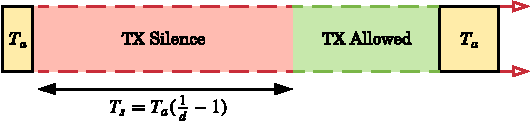
\includegraphics{Figures/duty_cycle_lorawan}
    \caption[\ac{lorawan} duty cycle enforcement]{
    Demonstration of how \ac{lorawan} enforces duty cycle limits; that is after a transmission of airtime $T_a$, the transmitter must be silent for a minimum period of $T_s=T_a(\frac{1}{d_c}-1)$ \cite{3YP:LIMITS_OF_LORAWAN}. The figure is to scale for $d_c=10\%$.
    }
    \label{fig:lorawan_duty_cycles}
\end{figure}

% Route management is the most researched challenge when it comes to ad-hoc networks \cite{3YP:MANET_RESEARCH_TRENDS} with implementations typically falling into the proactive or reactive categories - though more scenario specific variations do exist (e.g. geographic). Nodes using a proactive approach maintain a routing table for the whole network, to achieve this they rely on periodic updates from other nodes with their routing tables; these methods have low transmission delay but high ongoing overhead and adapt slowly to network changes. Nodes using a reactive approach explore the network when necessary to find a path, often by flooding route request packets; these methods have high transmission delay, but no ongoing overhead and can adapt to network changes immediately. Routing is not considered further in this paper so this is the abstracted level to which algorithms are considered. Full descriptions of many examples, including \ac{aodv} (reactive), \ac{olsr} (proactive) and \ac{lar} (geographic) can be found in \cite{3YP:ROUTING_ALGORITHMS}.